\documentclass[tikz,border=10pt]{standalone}
\usepackage{tikz}
\usetikzlibrary{arrows.meta,positioning}

\tikzset{
  card/.style={draw=blue!70!black, line width=1.2pt, rounded corners=3pt, minimum width=6.3cm, minimum height=1.0cm, align=center, fill=none},
  result/.style={draw=orange!80!black, line width=1.2pt, rounded corners=3pt, minimum width=6.3cm, minimum height=1.0cm, align=center, fill=none},
  flow/.style={-{Stealth[length=3mm]}, line width=1.2pt, draw=black!70}
}

\begin{document}
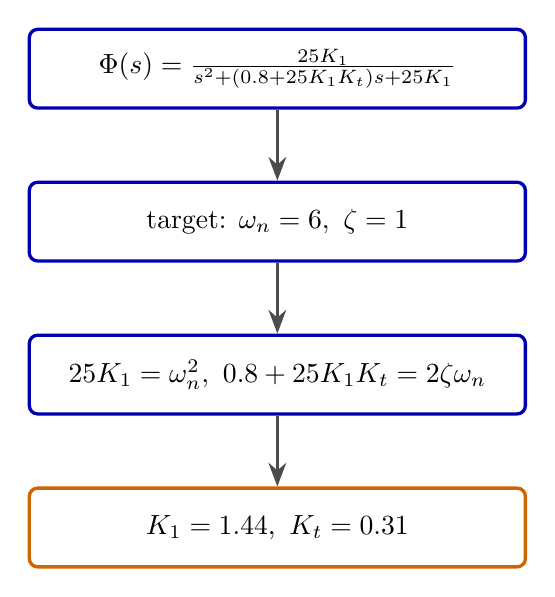
\begin{tikzpicture}[node distance=0.9cm]
  \node[card] (a) {$\Phi(s)=\frac{25K_1}{s^2+(0.8+25K_1K_t)s+25K_1}$};
  \node[card, below=of a] (b) {target: $\omega_n=6,\ \zeta=1$};
  \node[card, below=of b] (c) {$25K_1=\omega_n^2,\ 0.8+25K_1K_t=2\zeta\omega_n$};
  \node[result, below=of c] (d) {$K_1=1.44,\ K_t=0.31$};

  \draw[flow] (a) -- (b);
  \draw[flow] (b) -- (c);
  \draw[flow] (c) -- (d);
\end{tikzpicture}
\end{document}
